\documentclass{standalone}
\usepackage{tikz}
\usetikzlibrary{arrows.meta}

\begin{document}
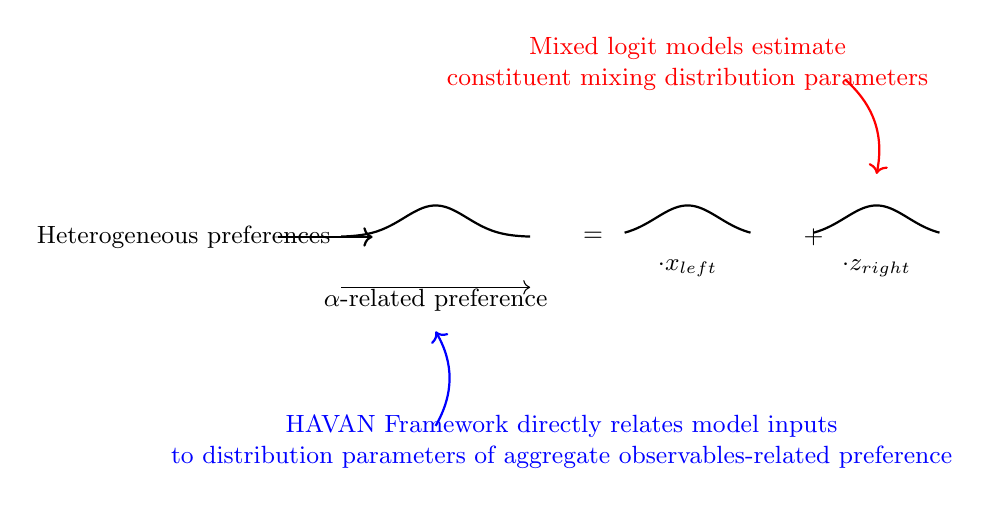
\begin{tikzpicture}[scale=0.8, every node/.style={font=\small}]

% Define Gaussian curve function
\newcommand{\gaussian}[3]{
  \draw[thick, domain=#1:#2, samples=50, smooth] plot (\x + #3, {0.5 * exp(-(\x)^2 / 0.5)});
}

% Left side: Heterogeneous preferences arrow and text
\node at (-5, 0) {Heterogeneous preferences};
\draw[->, thick] (-3.5, 0) -- (-2, 0);

% Left Gaussian curve
\gaussian{-1.5}{1.5}{-1}
\node at (-1, -1) {$\alpha$-related preference};
\draw[->] (-2.5, -0.8) -- (0.5, -0.8);

% Equals sign
\node at (1.5, 0) {$=$};

% Right side: First Gaussian with dot and x_left
\gaussian{-1}{1}{3}
\node at (3, -0.5) {$\cdot x_{left}$};

% Plus sign
\node at (5, 0) {$+$};

% Right side: Second Gaussian with dot and z_right
\gaussian{-1}{1}{6}
\node at (6, -0.5) {$\cdot z_{right}$};

% Top text and red arrow
\node[text=red] at (3, 3) {Mixed logit models estimate};
\node[text=red] at (3, 2.5) {constituent mixing distribution parameters};
\draw[red, ->, thick, bend left=30] (5.5, 2.5) to (6, 1);

% Bottom text and blue arrow
\node[text=blue] at (1, -3) {HAVAN Framework directly relates model inputs};
\node[text=blue] at (1, -3.5) {to distribution parameters of aggregate observables-related preference};
\draw[blue, ->, thick, bend right=30] (-1, -3) to (-1, -1.5);

\end{tikzpicture}
\end{document}